
\section{The One-World Feature of Kent's theory}
The third similarity Kent's theory shares with the pilot wave interpretation is that it is a one-world interpretation of quantum physics. It will be helpful to contrast this with the many-worlds interpretation. 

 Unlike the many-worlds interpretation, Kent's theory does not allow for indeterminate states of macroscopic objects such as cats. In the many-worlds interpretation, Schr\"{o}dinger will still only observe his cat to be either dead or alive, and not both dead and alive. However, Schr\"{o}dinger himself goes into a superposition of observing his cat to be alive and his cat to be dead. In the many-worlds interpretation, there is thus a difference between observing something to be so, and something actually being so: the observation is of a particular physical scenario, but the reality is a superposition of different physical scenarios. 

To capture this distinction between observation and reality, Bell speaks of \textbf{beables}\index{beable}.\label{beabledef} Bell introduces the term beable when speculating on what would be a more satisfactory physical theory than what quantum physics currently has to offer.\footnote{See \cite{Bell2}} Bell says that such a theory should be able to say of a system not only that such and such is observed to be so, but that such and such be so. In other words, a more satisfactory theory would be a theory of beables rather than a theory of observables. On the macroscopic level, these beables should be the underlying reality that gives rise to all the familiar things in the world around us, things like cats, laboratories, procedures, and so on. For example proponents of the pilot wave interpretation believe that the beables are all the particles each with their precise position and momentum. But whatever these beables are, it is because of them that a scientist can observe a physical system to be in such and such a state. Thus, observables are ontologically dependent on beables.   

Now the beables in Kent's one world interpretation are expressed in terms of a physical quantity called the \textbf{stress-energy tensor}\index{stress-energy tensor}  $T^{\mu\nu}(y)$.\label{stressenergy}   %
\nomenclature{$T^{\mu\nu}(y)$}{The stress-energy tensor, \nomrefpage}%
For any spacetime location $y$, the stress-energy tensor $T^{\mu\nu}(y)$ is an array of 16 values corresponding to each combination of $\mu, \nu=0,1,2,$ or $3$. %
\nomenclature{$\mu, \nu$}{Generic indices of tensors, $\mu, \nu=0,1,2,$ or $3$, \nomrefpage}%
 The value $T^{00}(y)$ is the energy density at $y$ divided by $c^2$,\footnote{This is not to be confused with the mass-energy density $T_S(x)$ defined for $x$ on a hypersurface $S$. As will be shown in section \ref{LorentzInvariance},   all 16 elements of $T^{\mu\nu}(x)$ will typically be needed to calculate $T_S(x)$.} whereas the other values of $T^{\mu\nu}(y)$ indicate how much energy and momentum flow across different surfaces in the neighborhood of $y$. 

It was mentioned in the previous section that for any spacetime location $x\in S$,  there is an observable $\hat{T}_S(x)$ acting on $H_S$ corresponding to the mass-energy density of the surface $S$ at $x$. It turns out that for any $\mu, \nu=0,1,2,$ or $3$, there is also an observable  $\hat{T}^{\mu\nu}(x)$ acting  %
\nomenclature{$\hat{T}^{\mu\nu}(x)$}{The observable corresponding to the stress-energy tensor $T^{\mu\nu}(y)$ in the Tomonaga-Schwinger picture, \nomrefpage}%
 on $H_S$, such that if $\ket{\Psi}\in H_S$ is a simultaneous eigenstate of $\hat{T}^{\mu\nu}(x)$ with eigenvalue $\tau^{\mu\nu}(x)$ for  %
\nomenclature{$\tau^{\mu\nu}(x)$ }{For fixed $\mu,\nu$, the simultaneous eigenvalue for all $x\in S$ of a simultaneous eigenstate $\hat{T}^{\mu\nu}(x)$, \nomrefpage}%
 all $x\in S$, then $\ket{\Psi}$ corresponds to a state of $S$ in which $T^{\mu\nu}(x)$ is  $\tau^{\mu\nu}(x)$ for all $x\in S$.\footnote{Note however, that such a simultaneous eigenstate is only for a fixed choice of $\mu$ and $\nu$, since in general, $\hat{T}^{\mu\nu}(x)$ and $\hat{T}^{\mu'\nu'}(x)$ will not commute for $\mu\neq\mu'$ or $\nu\neq\nu'$. } Moreover, the observable $\hat{T}_S(x)$ is expressible in terms of the  $\hat{T}^{\mu\nu}(x)$-observables.\footnote{See section  \ref{LorentzInvariance} for an explanation for why this is so.}\textsuperscript{,}\footnote{As in (\ref{approxeigen2}), we have the same implicit understanding of $\hat{T}^{\mu\nu}(x)$ and $\tau^{\mu\nu}(x)$ as being defined over cells $c_x\subset S$ rather than at spacetime locations $x\in S$, though we will often speak of them as being defined at spacetime locations. }
Now the  beables in Kent's theory are defined at each spacetime location $y$ that occurs after $S_0$ and before $S$. For such a spacetime location $y$, the beables will be determinate values of the stress-energy tensor $T^{\mu\nu}(y)$, but calculated from the expectation of the observable $\hat{T}^{\mu\nu}(y)$ conditional on the mass-energy density on $S$ being given by $\tau_S(x)$ for all $x\in S$ but outside the light cone of $y$. In section \ref{kentcalculation}, we will come back to the question of why we can't include any information about $\tau_S(x)$ for $x\in S$ within the light cone of $y$ when we discuss how these conditional expectations are calculated. But before we do that, we first consider why we should need conditional expectations at all in order to provide a one world description of reality.


To this end, we recall the definition of expectation in equation (\ref{expectation2}) and the expectation formula (\ref{evev}) for an observable. In a theory that posited the beables to be the expectation values of $\hat{T}^{\mu\nu}(y)$ for any $y$ located between $S_0$ and $S$  without conditioning on the value of the mass-energy density on $S$, then the $T^{\mu\nu}(y)$-beable would just be $\ev*{\hat{T}^{\mu\nu}(y)}{\Psi'}$ where $\ket{\Psi'}=U_{S'S_0}\ket{\Psi_0}$ for any hypersurface $S'$ that goes through $y$.\footnote{This can be done such that $\ev*{\hat{T}^{\mu\nu}(y)}{\Psi'}$ does not depend on the hypersurface $S'$ other than the fact that it contains $y$. For more details see \cite{SchwingerJulianI}.} However, such a beable would give a description of reality that was very different from what we observe. For instance, in a Schr\"{o}dinger cat-like experiment (see section \ref{SchrondingersCat}), there would be a stress-energy tensor distribution corresponding to both the cat being alive and the cat being dead in the same world as depicted in figure \ref{deadlivecat}.
\begin{figure}[ht!]
  \captionsetup{justification=justified}
  \centering
  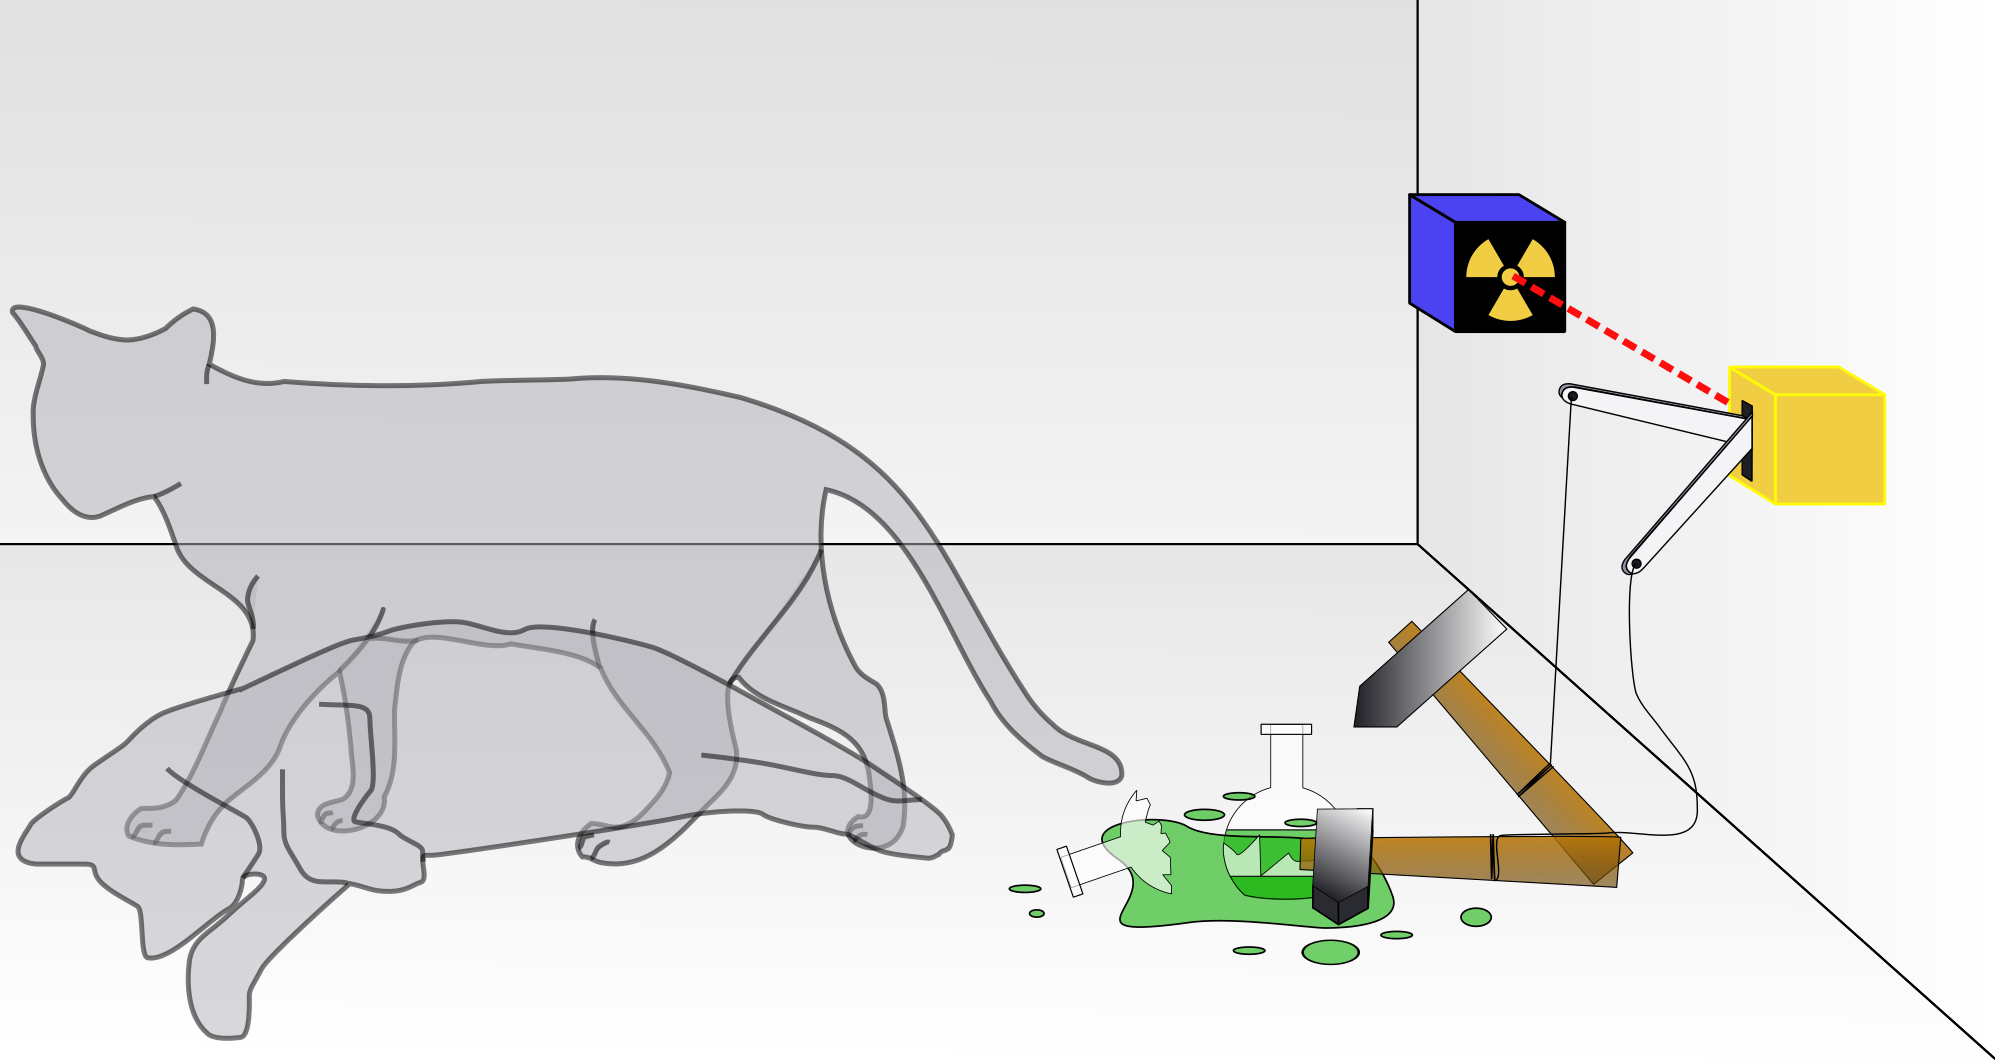
\includegraphics[width=100mm]{Chapter03/Schrodingers_cat.png}
  \caption[Caption for LOF]{A depiction of Schr\"{o}dinger's cat being both dead and alive.\protect\footnotemark}
  \label{deadlivecat}
  \end{figure}
  \footnotetext{ Original by Dhatfield. This image is licensed under the Creative Commons Attribution-Share Alike 3.0 Unported license. Source: https://commons.wikimedia.org/wiki/File:Schrodingers\_cat.svg}
  Such a distribution arises in this context because initially there is an atom that is in a superposition of decayed and non-decayed states, and so the expectation of $\hat{T}^{\mu\nu}(y)$ will have non-zero components both in the location where the non-decayed atom would be, and also in the locations of the decayed atom and the particle the atom emitted. As the decayed atom part of the state interacts with the poison releasing device, this device will also enter into a superposition so that in both the location of the poison containing flask and in the locations of all the poison atoms in the container containing the cat and into which the poison is released, the expectation of $\hat{T}^{\mu\nu}(y)$ will have non-zero components. And then the cat will enter into a superposition of being in a dead state and an alive state, and so  the expectation of $\hat{T}^{\mu\nu}(y)$ will have non-zero components in locations where the dead cat ends up and where the living cat happens to be. So the expectation of $\hat{T}^{\mu\nu}(y)$ in the locations of the container containing the cat will be very different from what someone would actually observe.


  To overcome this defect, information about the mass-energy density on $S$ is used, specifically the values of $\tau_S(x)$ for $x\in S^1(y)$ where  $S^1(y)$  %
  \nomenclature{$S^1(y)$}{The set  of all the spacetime locations of $S$ outside the light cone of $y$, \nomrefpage}%
  is defined to consist of all the spacetime locations of $S$ outside the light cone of $y$ as depicted in figure \ref{S2}.  

 \begin{figure}[ht!]
\captionsetup{justification=justified}
\centering

\tikzmath{
\a= 1;  
\e = 0.1;
\h=-1;
\hae=(3*\a*\a+6*\a*\e+7*\e*\e-3*\a*sqrt(\a*\a+4*\e*\e)-4*\e*sqrt(\a*\a+4\e*\e))/(4*\a+4*\e-2*sqrt(\a*\a+4*\e*\e));
\hae=0.0463647;
\hae=0.0858615;
\circsize=1.2;
\md = (\a+\h)/2;
\lrange = 4;
\rrange=2;
\ss=(-\lrange-\a)/2;
\sss=\a+(\rrange-\a)/2;
\tlen=0.75;
\labelpos=(-\lrange-\a)/2;
} 

\begin{tikzpicture}[thick, scale=2]

\def\dotsize{0.7}

\definecolor{tempcolor}{RGB}{0,151,76}
\draw[<->] (-\lrange, \h) node[left] {$S_0$} -- (\rrange, \h) node[right] {$S_0$};
\filldraw (0,0) circle (\dotsize pt) node [below right] {$y$} ;
              


\draw[<-] (-\lrange, \a)  -- (-\a, \a)  {};
\draw[gray, dotted] (-\a, \a) -- (0,0) {};
\draw[gray, dotted](0,0) -- (\a, \a) {};
\draw[->](\a, \a) --  (\rrange, \a)  ;         
\coordinate (B) at (\a,\a);
\node at (B)[red,circle,fill,inner sep=\circsize pt]{};
\coordinate (A) at (-\a,\a);
\node at (A)[red,circle,fill,inner sep=\circsize pt]{};
\coordinate (C) at (0,0);
\node at (C)[black,circle,fill,inner sep=\circsize pt]{};



\coordinate[label = above:$S^1(y)$]  (D) at (\ss,\a);
\coordinate[label = above:$S^1(y)$]  (D) at (\sss,\a);

\draw[->] (\rrange,\md-\tlen/2) --  (\rrange,\md+\tlen/2) node[midway,right]{time}; 
 
\node (start) at (\labelpos,\h) [below] {Initial State $\ket{\Psi_0}$};
\node (evolution) at (\labelpos,\md+0.05) [below] {Unitary Evolution $U_{S'S_0}\ket{\Psi_0}$};
\node (final) at (\labelpos,\a) [below] {Unitary Evolution $\ket{\Psi_S}=U_{SS_0}\ket*{\Psi_0}$};
%\node at (-\ss+0.17,\mn-0.18){$-a_0$};
\draw [->, shorten <= 5pt] (start) [above] -- (evolution); 
\draw [->] (evolution) -- (final); 
\end{tikzpicture}

\vspace*{2px}
\caption{The set $S^1(y)$ consists of all the spacetime locations of $S$ outside the light cone of $y$. The $T^{\mu\nu}(y)$-beables are calculated using the initial state $\ket{\Psi_0}$ together with the values of $\tau_S(x)$ for $x\in S^1(y)$. }
\label{S2}
\end{figure}
So in the case of Schr\"{o}dinger's cat, if the cat were dead,  light reflecting off the dead cat and going off into outer space would eventually intersect the hypersurface $S$, and the light distribution on $S$ would register the inanimate status of the cat. On the other hand, if the cat were alive, the light reflecting off the living cat and going off into outer space would also intersect $S$, but now the light distribution on $S$ would register the different locations the living cat was in as it moved about. Because light travels at a constant speed in a vacuum, the state of the cat at earlier times would be described by light distributions in regions on $S$ that were further away from the cat than those light distributions in regions of $S$ that described the cat in more recent times. 

Now if the cat was in a superposition of dead and alive states, then assuming there is no intermediate collapse of the global quantum state,  the hypersurface $S$ would also enter into a superposition of different states corresponding to these different distributions of light registered on $S$. But if a notional measurement on $S$ is made that determines which of these distributions is actually realized on $S$, then this determination will determine which history was actualized, and hence determine whether the cat actually survived Schr\"{o}dinger's experiment or whether it perished.   Thus, by conditioning on one of these two distributions on $S$ being actualized, the conditional expectation of the stress-energy tensor in the vicinity of where Schr\"{o}dinger's cat might be 
will not describe a situation like the one depicted in figure \ref{deadlivecat}.   Rather, it will either describe a situation like the one depicted in figure \ref{livecat}, or it will describe a situation like the one depicted in figure \ref{deadcat}. Which of these two situations occur will be determined by whether the measurement outcome on $S$ corresponds to a light distribution reflected from a living cat, or to a light distribution reflected from a dead cat. 
\begin{figure}[ht!]
  \captionsetup{justification=justified}
  \centering
  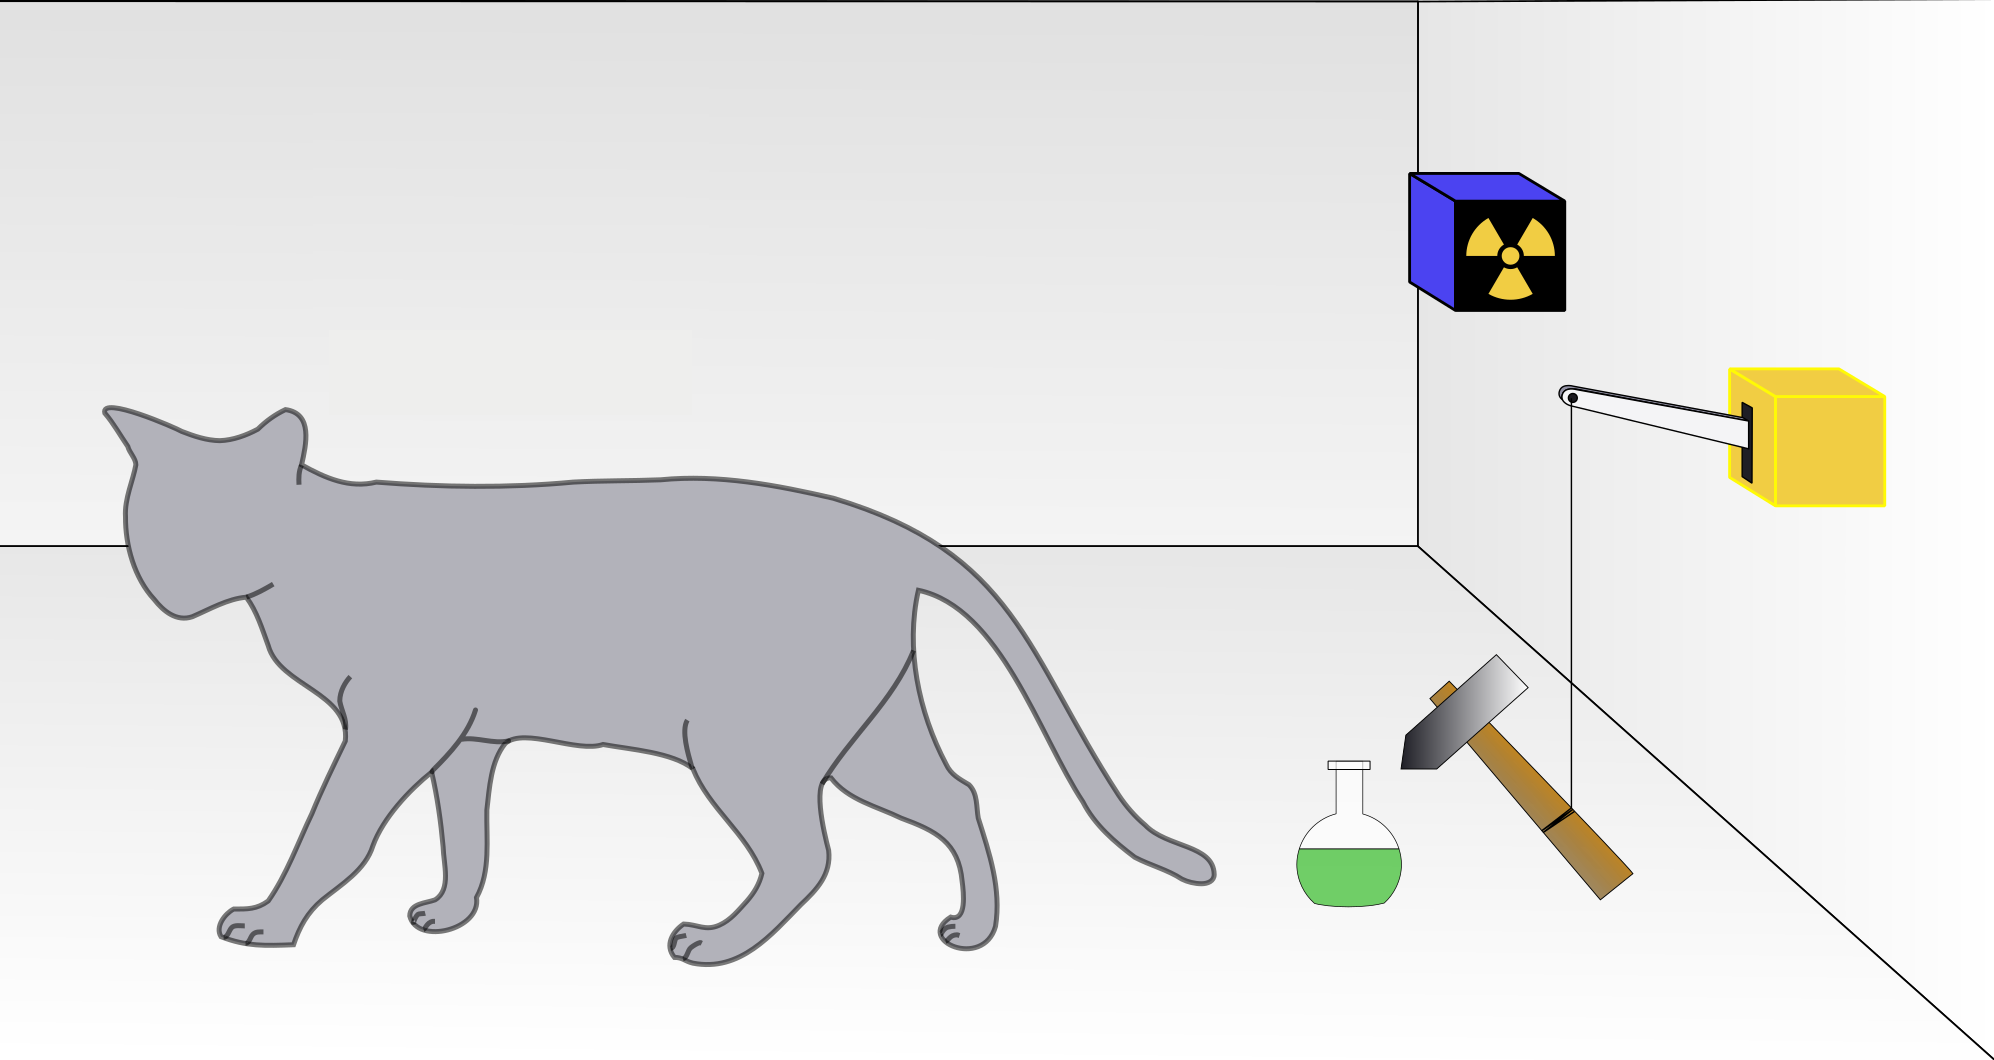
\includegraphics[width=100mm]{Chapter03/Schrodingers_livecat.png}
  \caption[Caption for LOF]{A depiction of Schr\"{o}dinger's cat being alive.\protect\footnotemark}
  \label{livecat}
  \end{figure}
  \footnotetext{ Original by Dhatfield. This image is licensed under the Creative Commons Attribution-Share Alike 3.0 Unported license. Source: https://upload.wikimedia.org/wikipedia/commons/archive/9/91/20080627113554!Schrodingers\_cat.svg}

  \begin{figure}[ht!]
    \captionsetup{justification=justified}
    \centering
    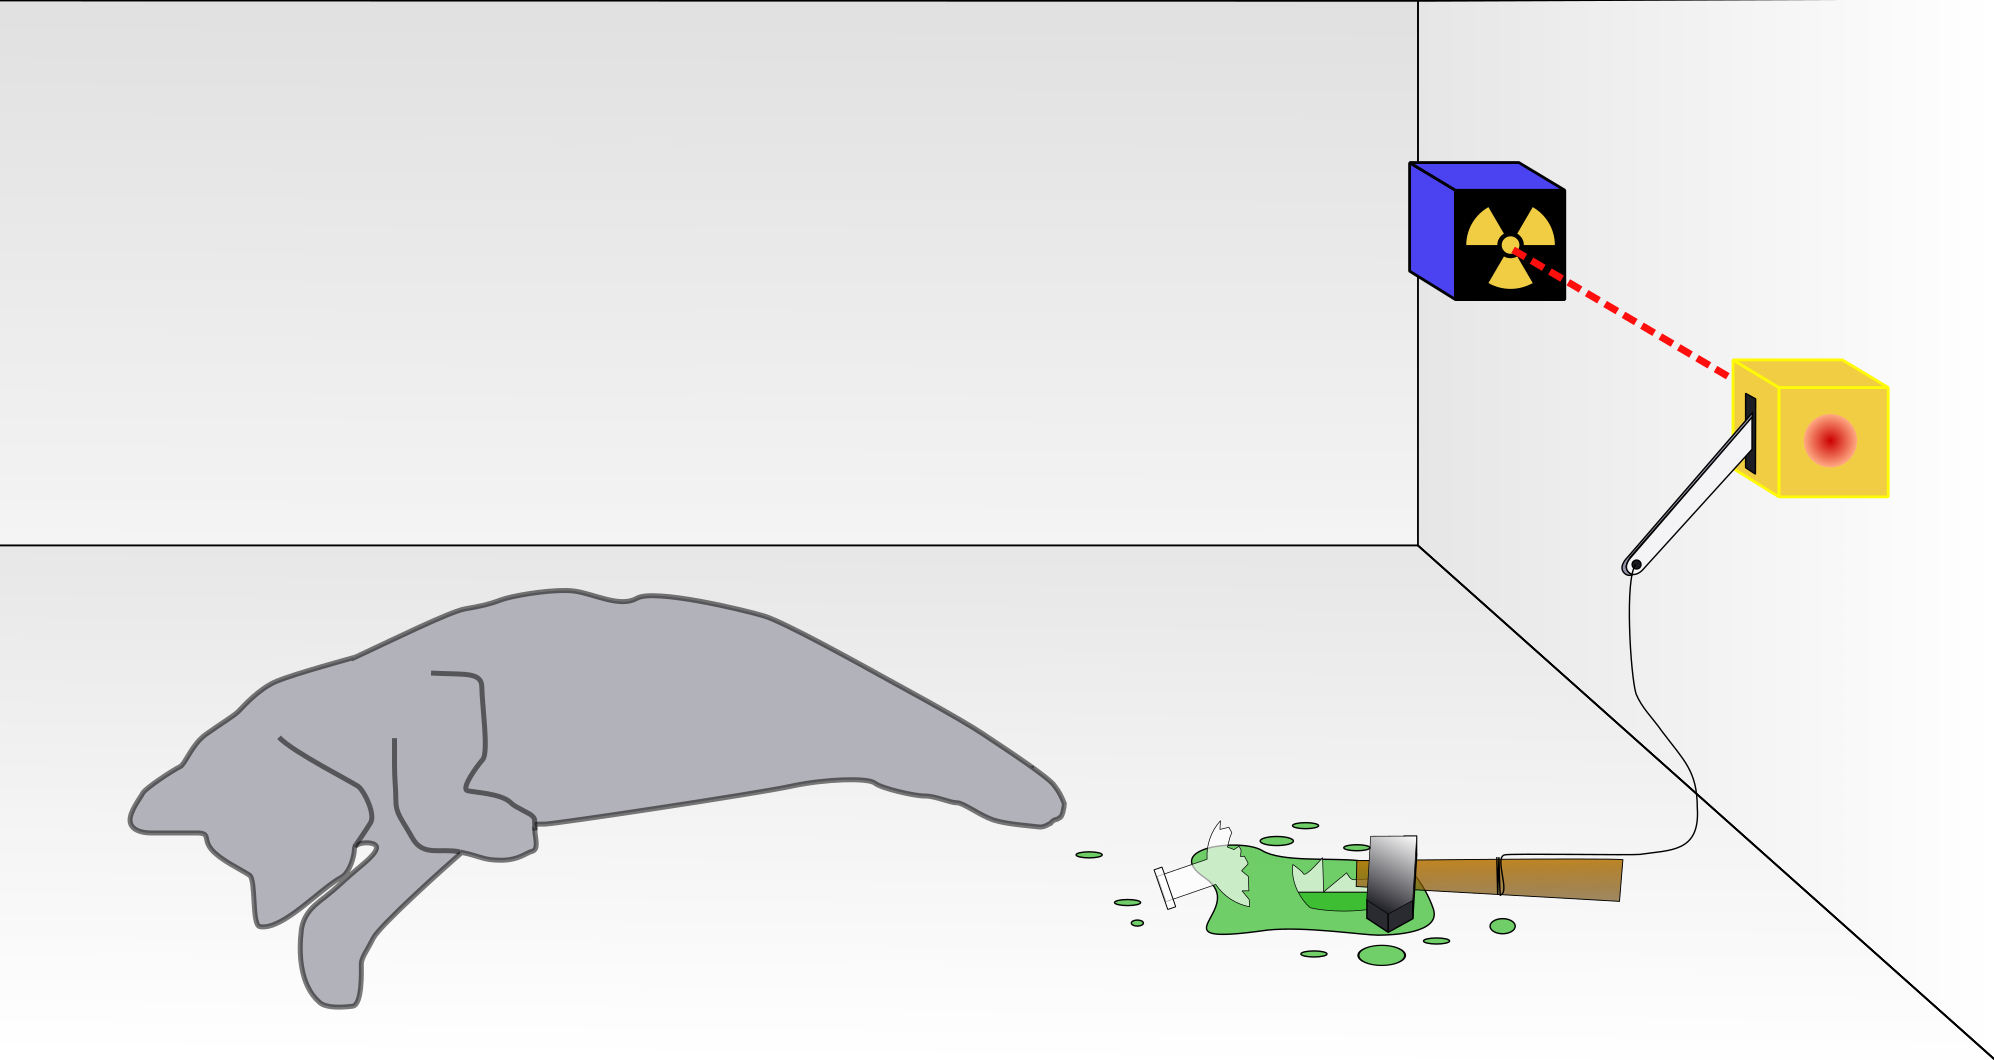
\includegraphics[width=100mm]{Chapter03/Schrodingers_deadcat.png}
    \caption[Caption for LOF]{A depiction of Schr\"{o}dinger's cat being dead.\protect\footnotemark}
    \label{deadcat}
    \end{figure}
    \footnotetext{ Original by Dhatfield. Altered by removing numbers and making into two separate figures. This image is licensed under the Creative Commons Attribution-Share Alike 3.0 Unported license. Source: https://upload.wikimedia.org/wikipedia/commons/archive/9/91/20080627113554!Schrodingers\_cat.svg}We assume that the outcome of the notional measurement (which determines which mass-energy distribution on $S$ is realized) occurs with a probability given by the Born rule. Under this assumption, we would then expect that in the history conditioned on this notional measurement, any scientists who performed measurements (in the normal sense of measurement) would measure average values of physical quantities consistent with the expectation values predicted by standard quantum theory. This intuition will be discussed in more detail in section \ref{KentconsistentQT}.
    
